\chapter*{\FontH{\Huge Meine Freundin Henna}}
\addcontentsline{toc}{chapter}{Meine Freundin Henna}
\lettrine[lines=3]{\color{red}D}{as} mutigste Mädchen, das ich kenne, heisst Henna. Sie ist meine beste Freundin. Mit ihr kann man immer tolle Sachen erleben. Wollt ihr die spannendste Geschichte hören, die ich je mit ihr erlebt habe? Also gut, ich erzähle sie euch.

Alles begann damit, dass meine Tante Susanne mal wieder was mit mir unternehmen wollte. Susanne ist erst siebzehn Jahre alt und ziemlich cool.Keine meiner Freundinnen hat eine so junge Tante. Von ihr weiss ich immer, welche Band gerade die beste ist und was es bedeutet, die Tage zu kriegen.

Sie hatte gerade furchtbaren Liebeskummer und wollte, wie sie sagte \enquote{deswegen} mit mir ein Schloss besichtigen. Was Liebeskummer mit einem Schloss zu tun haben könnte, weiss ich nicht, aber um ganz ehrlich zu sein, ich weiss schon nicht einmal, was Liebeskummer bedeuten soll. Das macht aber offenbar nichts, denn wenn mir Susanne von ihrem Liebeskummer erzählt, presse ich die Lippen zusammen, gucke so wie Papa, wenn er von seiner Arbeit spricht und nicke dazu. Susanne findet, dass ich die einzige bin, die sie versteht.

Und eine Freundin solle ich mal auch mitnehmen, hat Susanne vorgeschlagen, dann werde es um so lustiger. Und damit hatte sie Recht. Bei so einer Einladung kam nur Henna in Frage. Da musste ich gar nicht lange überlegen. Wir drei vereinbarten, uns gegen späten Nachmittag beim Schloss zu treffen.

Schon gleich nach der Kasse begannen unsere Probleme, ohne das Henna und ich das aber wissen konnten. Ein junger Mann im Alter von Susanne stand hinter uns und irgendwie sind die beiden ins Gespräch gekommen. Die ersten beiden Räume, die wir im Schloss besichtigten, stand er die ganze Zeit neben uns. Die beiden waren sehr albern, viel alberner als wir. Dann entschuldigten sich er und Susanne, sie würden gerne einen Kaffee im Museum in der Nähe des Schlosses trinken gehen wollen. Wir genehmigten gerne und machten uns auf den Weg durchs Schloss.

Das Schloss war wunderschön und könnte auch genauso in einem Märchenbuch gemalt worden sein. Hohe spitze Türme an allen Seiten, ringsherum ein Park, der mit einer hohen Mauer umgeben war. Wie bei einer Burg. Und überall Rosen. Die Zimmer waren laut Tafeln so, wie sie früher dann und dann gemäss der Phantasie des Schilderschreibers gewesen sein müssen. In jedem Zimmer ein Kachelofen und dann überall Rüstungen, Waffen und Besteck von damals. Wenn ich so ein Schloss gehabt hätte, hätte ich die Sachen wohl anders aufbewahrt, aber die Menschen früher haben sich wohl noch nicht so viele Gedanken gemacht wie wir jetzt. Das merke man schon daran, was sie für ein WC gehalten haben, meinte jedenfalls Henna, und da hatte sie Recht. Denn das WC war nur ein Erker in der Wand mit einem Loch. Henna und ich haben dort durchgespuckt und uns vorgestellt, was da sonst schon alles runtergefallen ist. Ob es wohl sehr umständlich war für einen Ritter, jedesmal die Rüstung abziehen zu müssen, wenn die hierher gekommen sind?

Wir sind in jedem Raum gewesen und haben uns immer eine Geschichte zu den Dingen überlegt, die da so standen. Henna meinte, dass die Menschen, die früher hier gelebt haben, noch an Zauberei, Drachen und Gespenster geglaubt haben. In einem Zimmer lag unter einer Vitrine ein sehr grosses aufgeschlagenes Buch, mit Buchstaben, die wir nicht lesen konnten. Das haben wir für ein Zauberbuch gehalten und uns gerade gefragt, ob das Buch selber zaubern kann oder ob man die die Zaubersprüche erst vorlesen muss. Gerade als wir ausprobieren wollten, ob wir den ausgestopften Vogel in einem Regal wieder lebendig zaubern können, hörten wir ein lautes Krachen von draussen.

Eigenartigerweise ist in dem Schloss niemand zu sehen, als wir raus liefen, um nach zu sehen. Auch im Park ist keine Menschenseele, dabei waren es noch so viele, als wir gekommen waren. Das grosse Tor durch die Mauer ist zu. Eine schwere Holztür ist da, wo wir rein gekommen sind. Das Schliessen des Tores hat wohl den Krach gemacht, den wir gehört hatten, schlussfolgert Henna. Sofort fangen wir aus Laibeskräften an zu rufen. Aber niemand hört.

Henna unterbrach mich, es habe keinen Sinn so zu schreien. Auf ihren Rat hin liefen wir der Mauer entlang, um nachzusehen, ob wir nicht sonst irgendwo raus kommen, denn raus wollten wir hier. Das ist sicher. So eine Nacht in einem Schloss verbringen? Ganz alleine? Und wo war eigentlich Susanne? Offensichtlich war jetzt Feierabend hier im Schloss, das Museum ist geschlossen worden und uns haben sie vergessen.

Aber da ist kein anderes Tor und keine Lücke. Die Mauer ist dicht, da kommt niemand rein, dass haben die damals schon richtig gemacht, aber es kommt eben auch niemand raus. Henna meint, in jedem Schloss gebe es geheime Fluchtwege. Man müsse nur in der Bibliothek an einem bestimmten Buch ziehen, dann drehe sich die Wand und man kommt in einen unterirdischen Tunnel. Das haben alle Schlösser, das kenne sie aus dem Fernsehen.

Wir haben in allen Zimmern nach der Bibliothek gesucht, aber keine gefunden. Wir kommen noch gar nicht dazu, uns Gedanken zu machen, wie wir jetzt weiter machen, nachdem wir keine Bibliothek gefunden haben, denn wir werden von einem lauten Schlag erschreckt. Ein Donnern, der durch das ganze Schloss dringt.

Ich bleibe wie angewurzelt stehen, aber Henna meint, das sein nur die Eingangstüre, die hätten wir offen gelassen und ein Windstoss habe sie zugeschlagen.

Da hat sie schon wieder Recht, denn es ist auch ganz still geworden. Mit geschlossener Tür ist nichts mehr zu hören, ausser wie Henna atmet. Sie ist Allergikerin, wahrscheinlich waren gerade irgendwelche Pollen in der Luft. Noch schlimmer ist es bei Katzen. Katzenhaare merkt Henna sofort. Wenn ich die Katze von Susanne streichele und dann Henna besuche, muss sie sofort husten.

Es ist nicht nur still, sondern mit der Zeit auch dunkel geworden, denn die Sonne ging nun unter. Eine Rüstung hatte so einen langen Schatten geworfen, dass es aussah, als müsste irgendwo ein Riese stehen mit Schild und Schwert. Mir wurde es sehr flau im Magen, ich hatte ein bisschen Angst, denn Schlösser können, so schön sie am tag auch sind, nachts ziemlich unheimlich werden. Deswegen werden die wohl auch abends geschlossen, nehme ich an. Ob Susanne überhaupt bemerkt hat, dass wir weg sind? Henna und ich versuchen einen Lichtschalter zu finden. Aber entweder sind die sehr gut versteckt, oder hier machen die noch Licht mit Kerzen. Jedenfalls suchten wir neben jeder Tür nach einem Schalter, zu Hause bei mir und bei Henna und bei jedem, den wir kennen, sind alle Lichtschalter neben einer Tür.

Ich überlegte gerade, wie das bei Onkel Tonis Stall ist, der ist auch ziemlich gross, so wie das Schloss und vielleicht ist das mit den Lichtschaltern ja anders in grossen Gebäuden. In dem Augenblick hörten wir ein leises Tapsen einen Stock über uns. Wäre es nicht so gruselig still gewesen und würde es in so einem Schloss nicht so hallen, hätten wir das nie gehört. Haben wir aber. Mir wäre fast das Herz in die Hose gerutscht und ich halte die Luft an, um blos selber kein Geräusch zu machen. Erstens konnte ich so besser hören und zweitens konnte ich selber so nicht gehört werden. Auch Henna lauscht gespannt.

\afterpage{
    \begin{figure}
        \thispagestyle{empty}
        \centering
        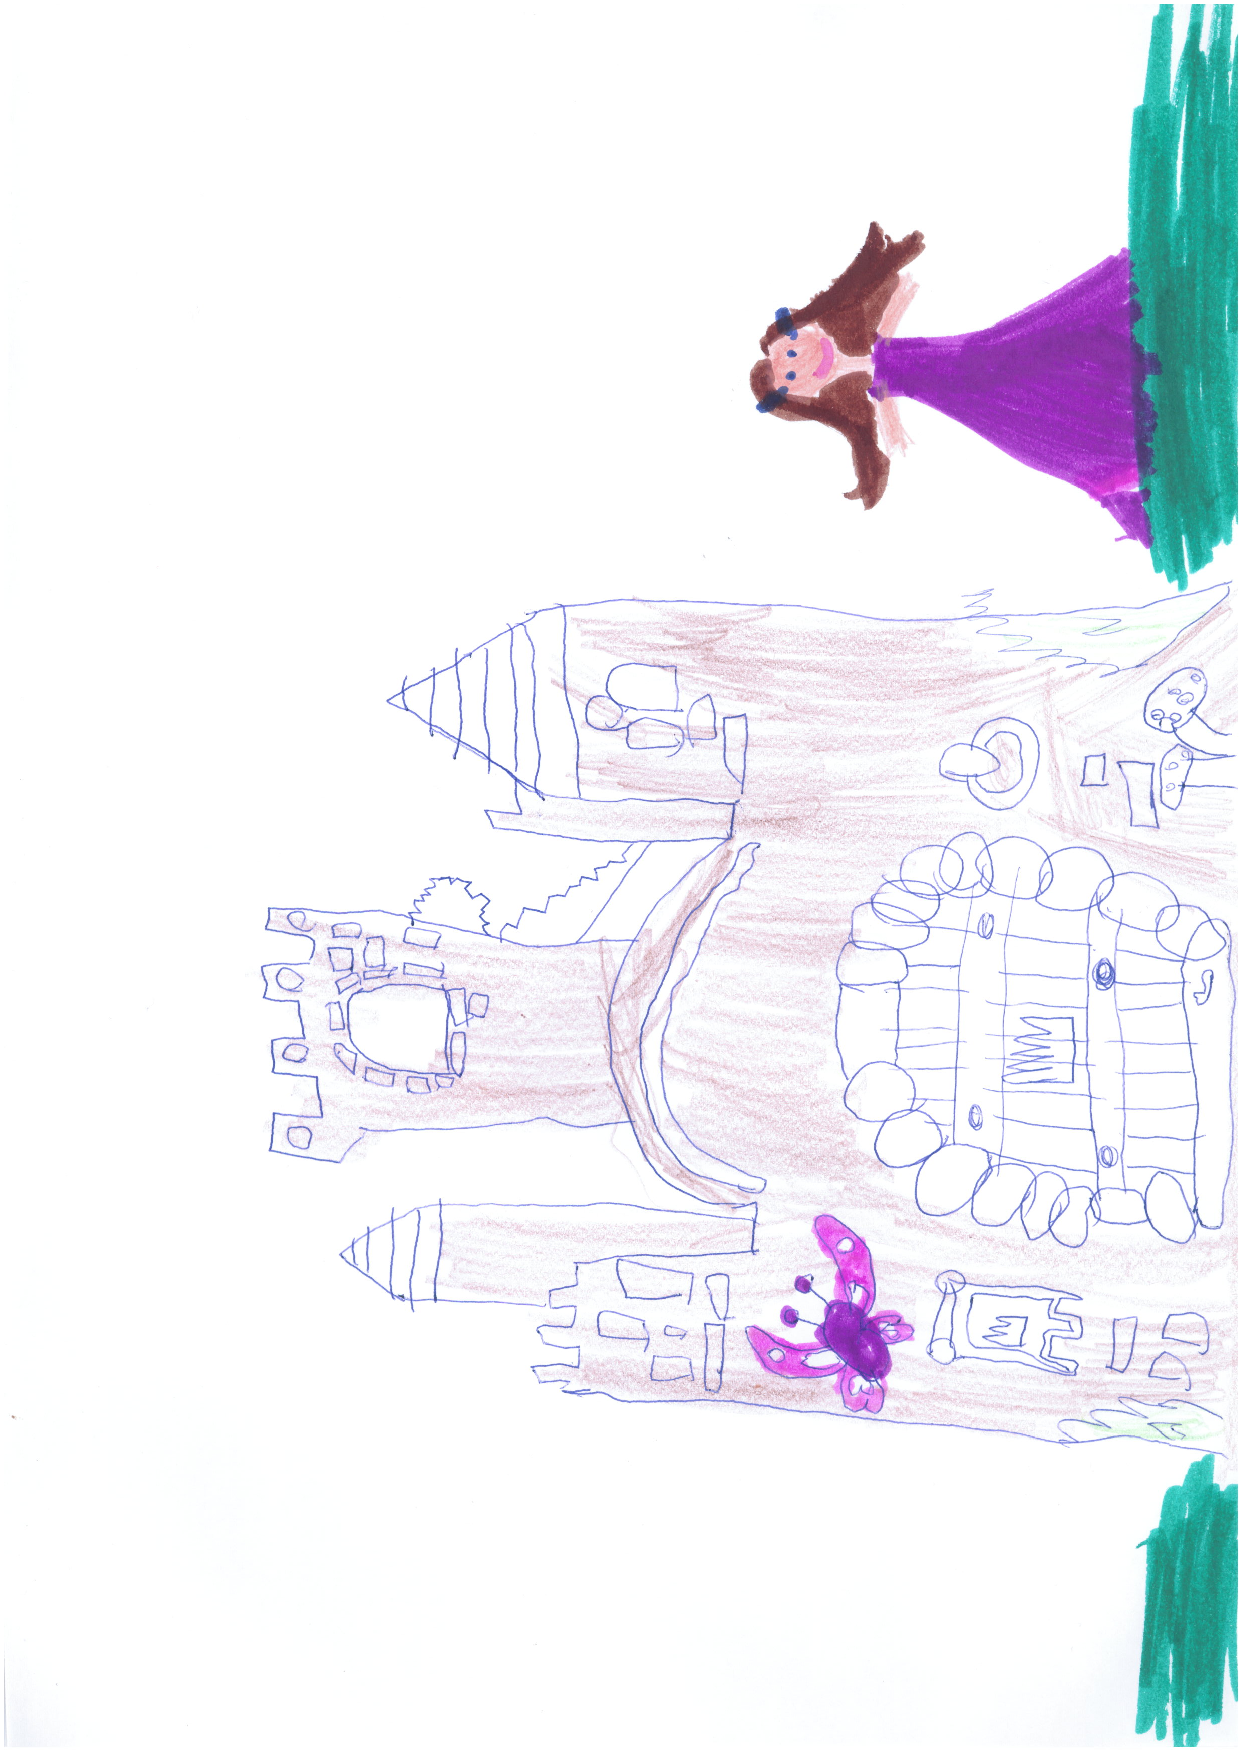
\includegraphics[angle=270,width=\textwidth]{bilder/prinzessin.pdf}
    \end{figure}
    \clearpage
}

Was ist jetzt besser? Laut rufen, vielleicht ist da ja irgendwo Susanne und sucht uns oder lieber ganz leise sein und sich verstecken? Ich entschied mich gerade für die zweite Variante, denn wie von Susanne hat das Geräusch nicht geklungen. Na ja, das Geräusch hat eigentlich überhaupt nicht nach einem Mensch geklungen.

Aber Henna macht meinen Plan kaputt. Sie ruft ganz laut, ob da jemand sei. Ich bin sehr erschrocken von der Lautstärke und von dem Echo. Niemand antwortet. Henna ruft nochmals. Nichts. Doch dann war wieder das Tapsen zu hören. Henna läuft sofort los um nachzusehen. Ich habe viel zu viel Angst, hier alleine stehen zu bleiben, also folge ich ihr. Die Treppe hoch, dort kam das Geräusch her. Mir bleibt fast das Herz stehen. Das Tapsen ist ganz klar aus dem Zimmer am Ende des Ganges zu hören. Der Mond scheint sehr hell, es ist zwar alles zu erkennen, aber nur schwarzweiss. Das ist mir da zum ersten Mal aufgefallen, dass alle Dinge nachts grau werden. Henna geht zielstrebig auf das Zimmer zu. Mein Herz schlägt so laut, als ob irgendjemand ganz laut Musik spielt. Ich bin sicher, dass mindestens Henna das hören muss und wer immer da drin ist auch. Wenn die Menschen, die hier gewohnt haben an Gespenster geglaubt haben, dann hatten die womöglich doch Recht. Sind Gespenster eigentlich gefährlich? In Trickfilmen ja meistens nicht, aber ob man sich auf Trickfilme verlassen kann, ist ja wohl fraglich. Ich meine, da fallen ja auch sprechende Tieren Klaviere auf den Kopf und denen passiert nichts. 

Wir näherten uns dem Zimmer. Ich weiss nicht, warum genau wir eigentlich nachsehen wollten und ob es nicht besser gewesen wäre, sich zu verstecken und das wollte ich Henna aucg gerade sagen, da ist sie schon in dem Zimmer und um die Ecke. Ich schnell hinterher. Das Tapsen kam vom anderen Ende des Zimmers. Der Mond schien durch das Fenster, aber um in jede Ecke zu gucken reichte das Licht nicht. Da ist es entweder ganz schwarz oder ein Wirrwarr aus Schatten, dass man nichts erkennen kann.

Plötzlich bewegte sich einer dieser Schatten und wird länger und immer länger und so lang, dass er erst bis zur Wand hinter unserem Rücken reichte und dann war ein lauter Schlag zu hören, viel lauter und heller als der vorhin und tausende Scherben fliegen uns entgegen. Irgendetwas ist kaputt gegangen. So etwas wie eine riesige Tasse oder so, jedenfalls sahen die Scherben so aus.

Ich traute mich nicht einmal mit den Wimpern zu schlagen. Henna sprang aber nach vorne und greift zu. Ein Fauchen war zu hören. Ich konnte das alles nicht so richtig erkennen, aber ich hörte Henna rufen: \enquote{Übel, ganz übel \dots eine Katze!}

Und tatsächlich hielt sie eine Katze im Arm. Wie ihr euch vorstellen könnt, bin ich noch nie im Leben so erleichtert gewesen wie da. Kein Gespenst, kein Vampir, kein Einbrecher oder sonst etwas Schreckliches. Nie wäre ich auf die Idee gekommen, dass es eine Katze sein könnte! Henna sah das anders. Sofort fing sie an zu husten. Ich nahm ihr die Katze ab und scheuchte sie raus. Die muss wohl rein gekommen sein, als wir die Tür aufgelassen hatten.

Henna fand ein ein richtiges WC, so ein eins für Besucher, da hat sie sich die Hände gründlich gewaschen. Dann ging es mit dem Husten auch gleich besser. Dann haben wir noch geflucht, nichts zum Essen zu hatten, nur Wasser aus der Leitung gab es hier. Das Bett der Königin hat uns dann aber wieder versöhnt. Riesig und ein Himmelbett noch dazu. Die Decke goldbestickt, aber sehr muffig. 

Dort haben wir gerade geübt, wer am höchsten springen kann und bis an die Spitze des Himmelbetts kommt, als wir das Rufen von Stimmen hören. Die von Susanne ist auch dabei. Dazu noch jemand, der der Hose nach der Hausmeister sein könnte. Der Typ von vorhin ist auch dabei. Susanne entschuldigt sich tausend Mal, der Hausmeister will immer wieder wissen, ob wir etwas angefasst hätten und droht mit der Polizei, als er die umgestürzte Vase fand. Die Katzengeschichte will er uns nicht glauben, hier wäre noch nie eine Katze gewesen. Aber das ist jetzt alles nicht mehr unser Problem, dass muss jetzt wirklich Susanne lösen.

Wir vier gehen dann noch in eine Pizzeria und es wird noch ein sehr lustiger Abend. \hfill {\color{red}\decofourleft}




